\subsection{Visualisierungsmöglichkeiten und Zielgruppe}
\label{sub:visualisierungsmöglichkeiten_und_zielgruppe}
  Die Recherchearbeit führte  zu einer Sammlung an verschiedensten Materialien. Live-Karten, Plugins, Tube-Maps aber auch wissenschaftliche Arbeiten die an das eigene Thema angrenzen wurden gesucht und in verschiedene Listen übernommen. In Abbildung \ref{fig:viz_overview} ist ein Teil dieser Materialsammlung zu sehen.

  \begin{figure}[htbp]
    \begin{center}
      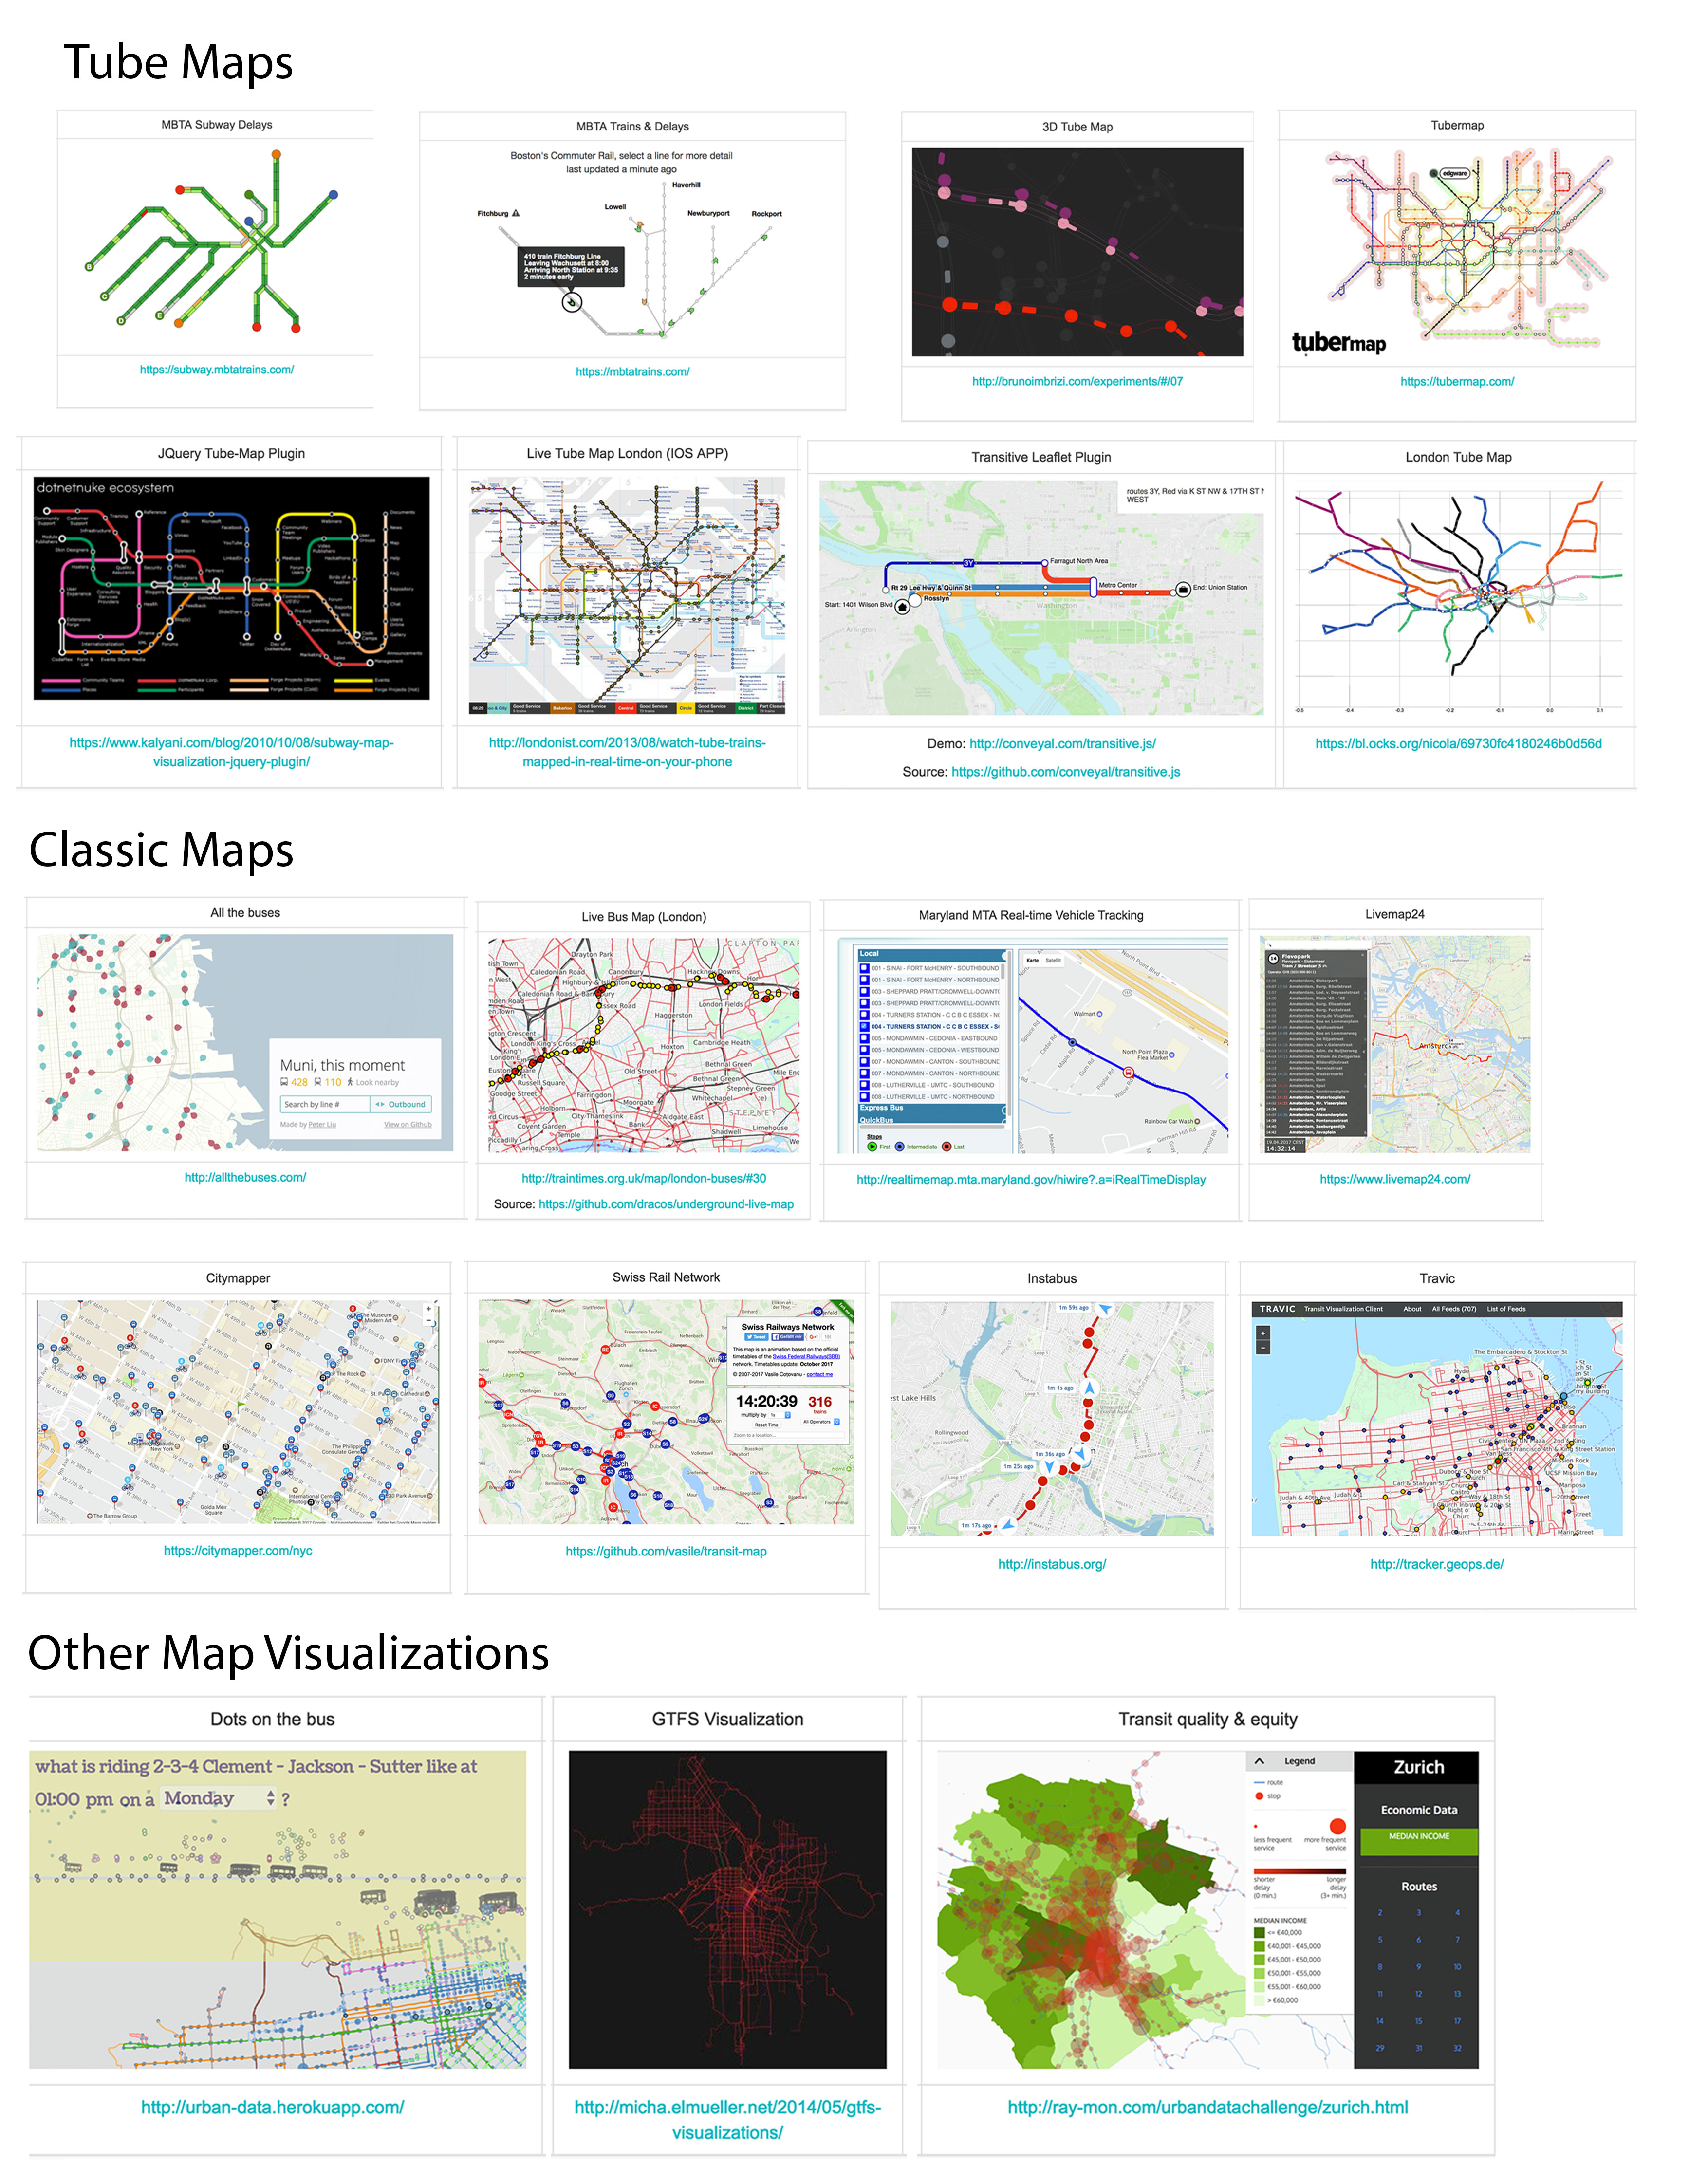
\includegraphics[width=0.5\textwidth]{viz_overview}
      \caption{Überblick über bestehende Tools und Visualisierungen}
      \label{fig:viz_overview}
    \end{center}
  \end{figure}

  Das gesammelte Material zu den möglichen Visualisierungsarten wurde in einer 2x2 Matrix (Abbildung \ref{fig:2x2_matrix}) in die Unterkategorien "`Live-Karten, Künstlerische Visualisierung, Plugin / Software / Tool, Tube-Map"' eingeordnet, um einen sortierten Gesamtüberblick zu bekommen. 

  \begin{figure}[htbp]
    \begin{center}
      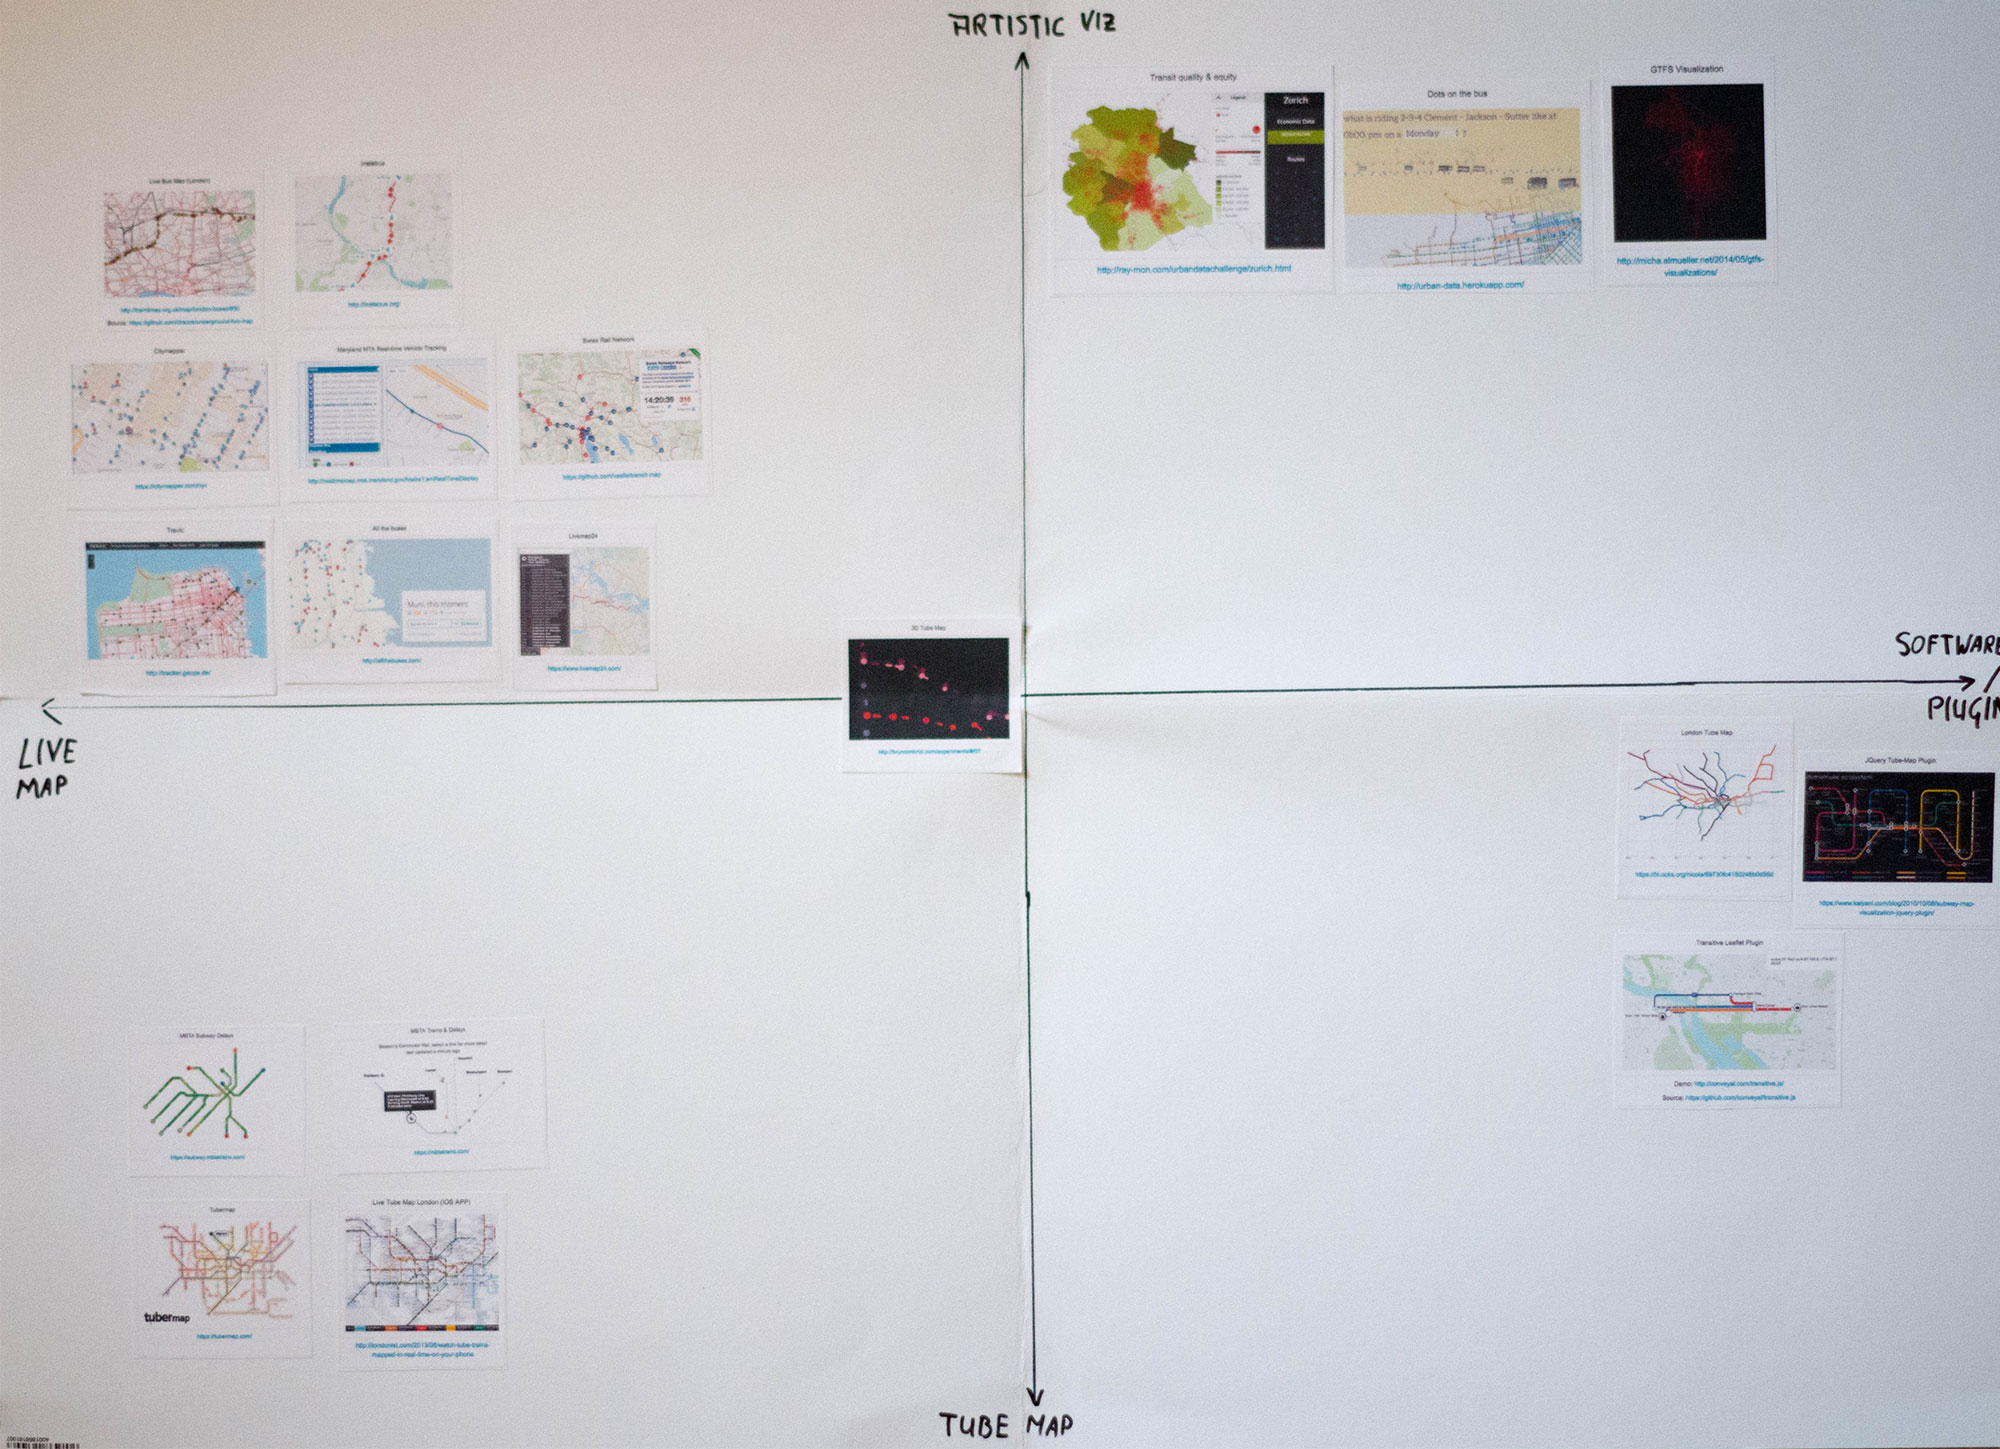
\includegraphics[width=0.4\textwidth]{2x2_matrix}
      \caption{2x2 Matrik Methode auf DIN A2}
      \label{fig:2x2_matrix}
    \end{center}
  \end{figure}

  Durch diese Ansicht wurde die Erkenntnis gewonnen, dass es schon viele Live-Visualisierungen auf interaktiven Karten gibt, aber nur sehr wenig so genannte Tube-Maps. Auch sind bereits verschiedenste Tools zum Generieren von GTFS-basierten Visualisierungen vorhanden. Eine sehr ausführliche, aber bei weitem nicht vollständige Liste über das Thema "`Transit"' wurde auf Github von der Community zusammengetragen \url{https://github.com/luqmaan/awesome-transit}.

  Damit die verschiedenen existierenden Zielgruppen besser verstanden werden können, wurden sogenannte \texttt{Personas} eingesetzt\parencite{personas}. Personas sind fiktive Charaktere, die auf der Grundlage von Recherche erstellt werden, um die verschiedenen Benutzertypen eines Produktes oder Service zu simulieren. Sie können dabei helfen, einen Perspektivenwechsel zu vollziehen und sich in verschiedene Nutzer hineinzuversetzen, um ihre unterschiedlichen Bedürfnisse, Ziele und Erwartungen besser zu verstehen.
  Für die Charakterisierung werden typische Merkmale, Stereotype oder Trends genutzt. Wie in Abbildung \ref{fig:personas} zu sehen ist, wurden in der Recherche-Phase drei mögliche Nutzergruppen identifiziert.

  \begin{figure}[htbp]
    \begin{center}
      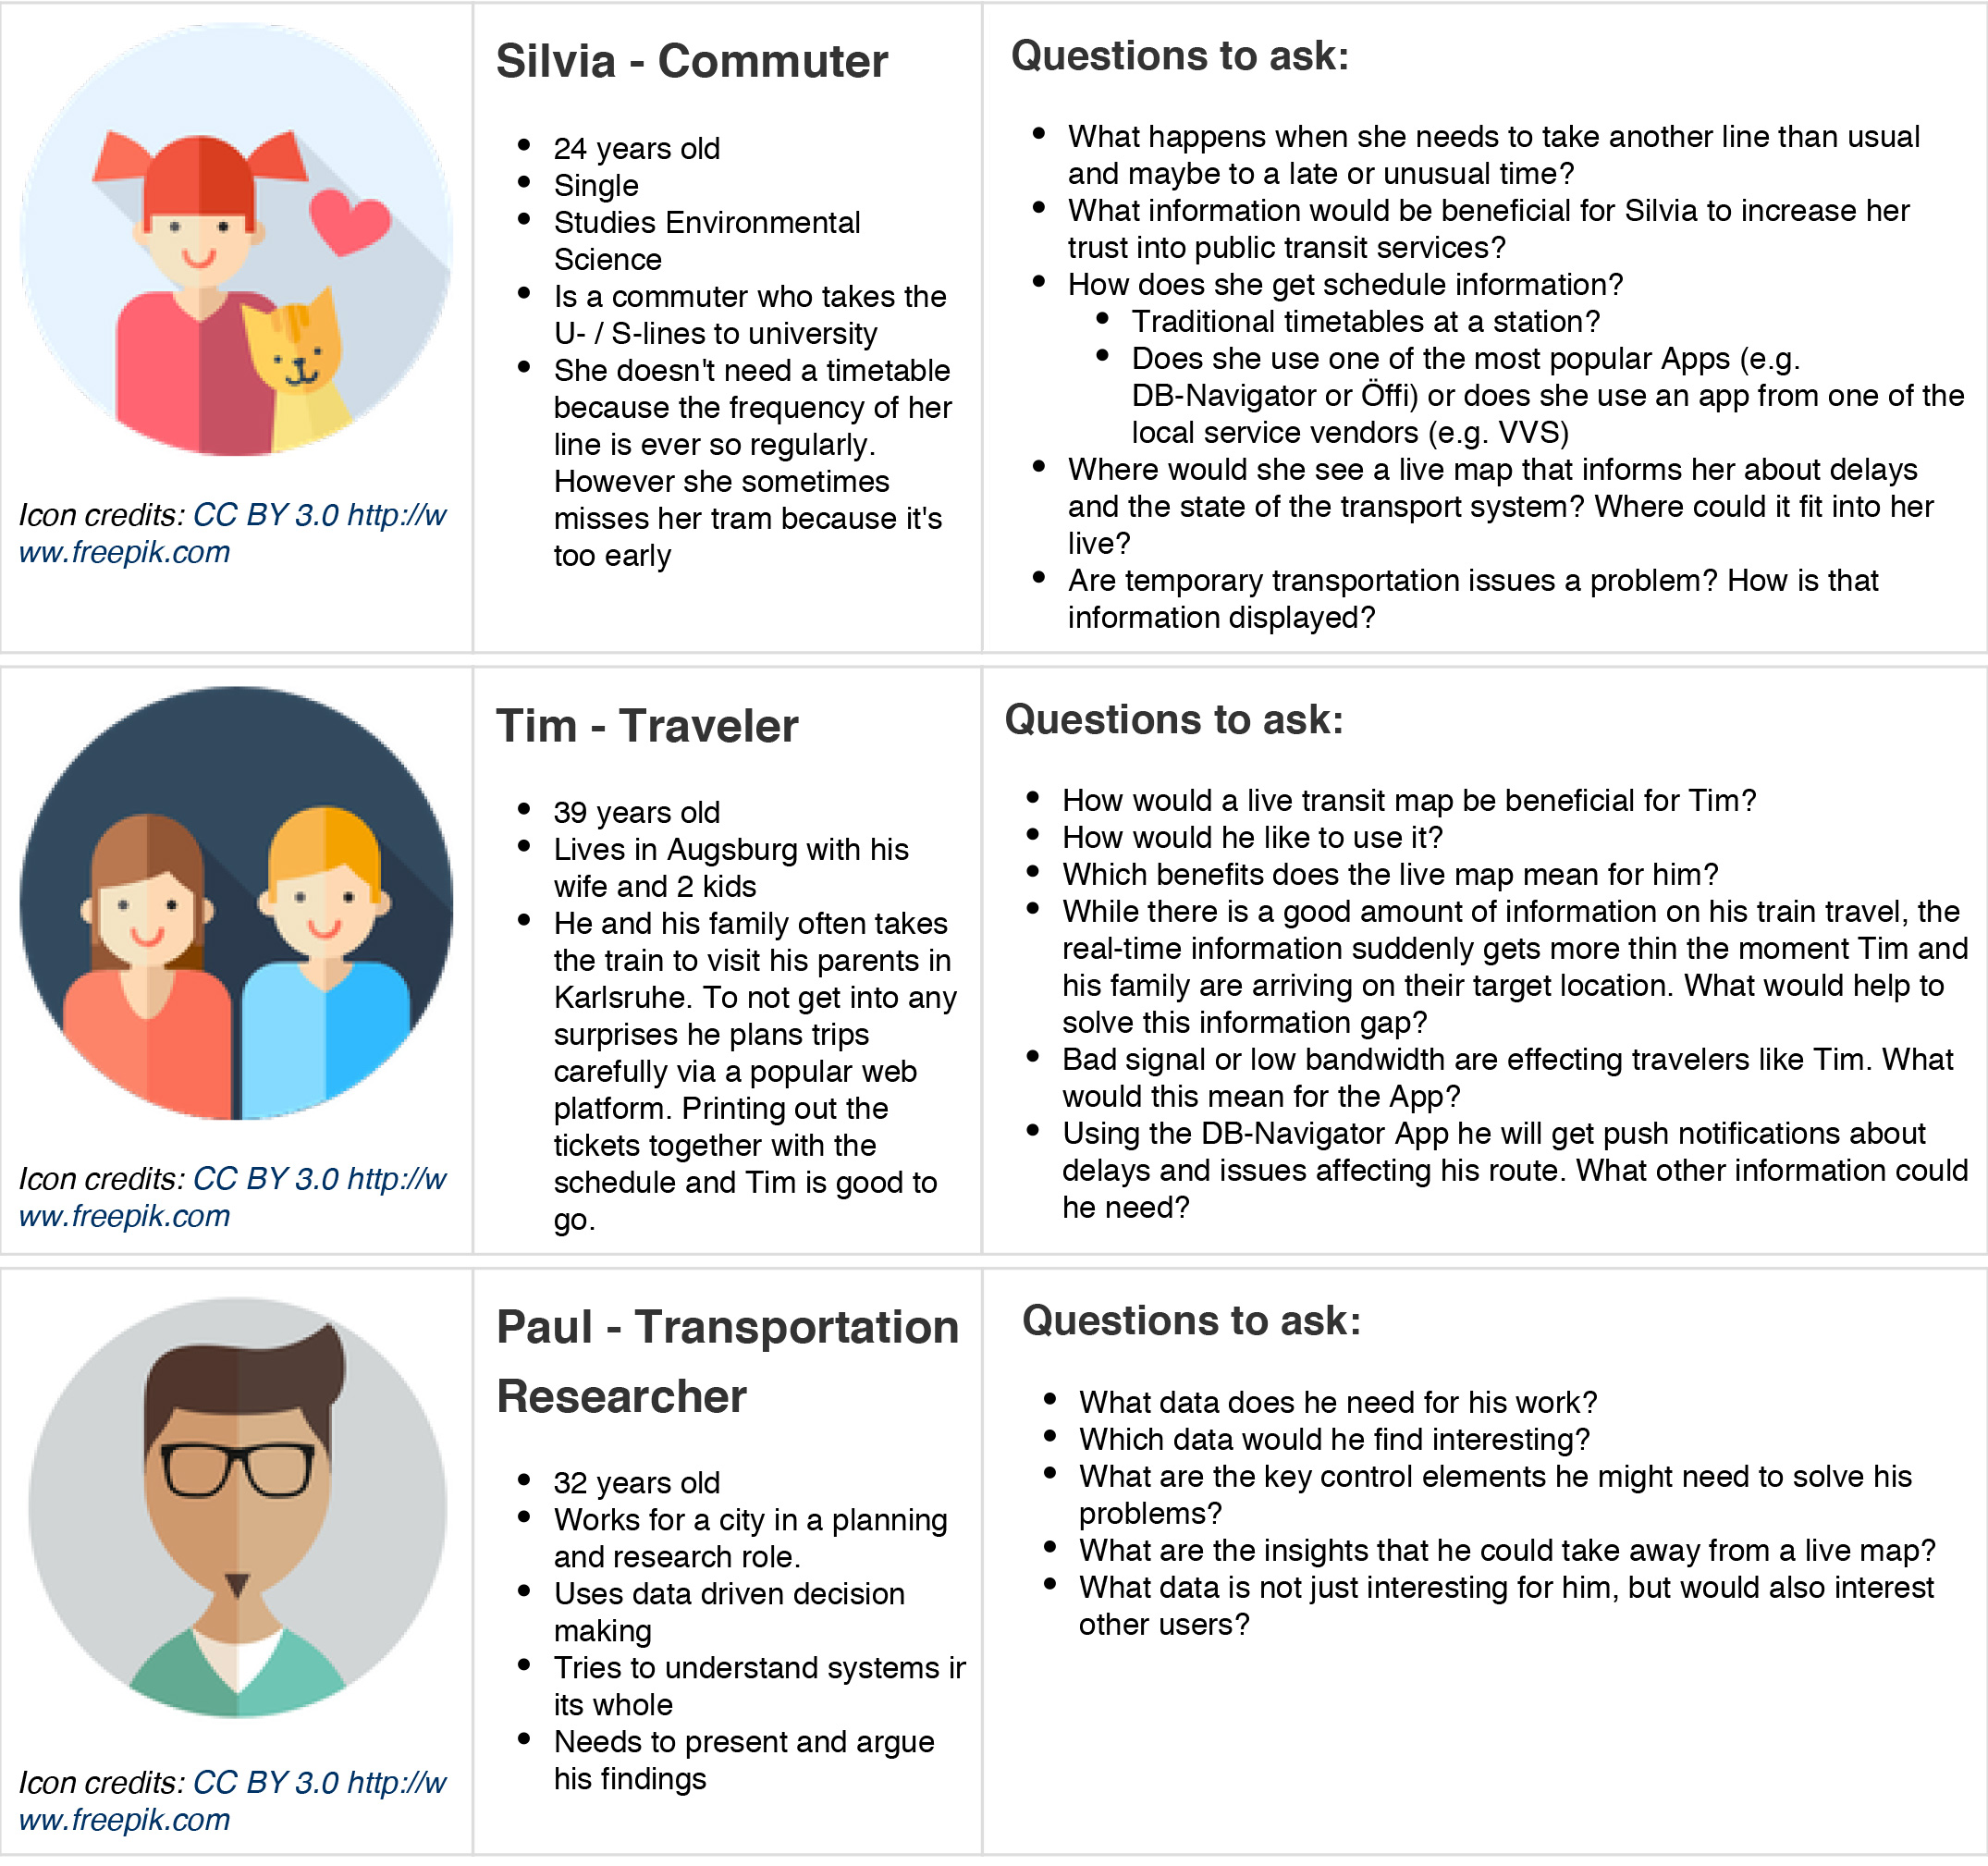
\includegraphics[width=0.9\textwidth]{personas}
      \caption{Personas}
      \label{fig:personas}
    \end{center}
  \end{figure}

% subsection visualisierungsmöglichkeiten_und_zielgruppe (end)